\section{Methods}
\label{sec:methods}

To compute the coarse matrix $Ac$, a triple matrix multiplication should be done:
\begin{equation}
 Ac = R \times A \times P
\end{equation}
in which $R = P^T$. We do it in two parts, performing matrix-matrix multiplications (\matmult) twice: first $A \times P$, then $R \times B$, in which $B = A \times P$.

The matrices are partitioned on multiple processors by row blocks (Figure~\ref{fig:partition}). Matrices $A$ and $P$ have the same number of rows and consequently are partitioned the same way. $R$ has less number of rows and has a different partition.

\begin{figure}[tbh]
 \centering
 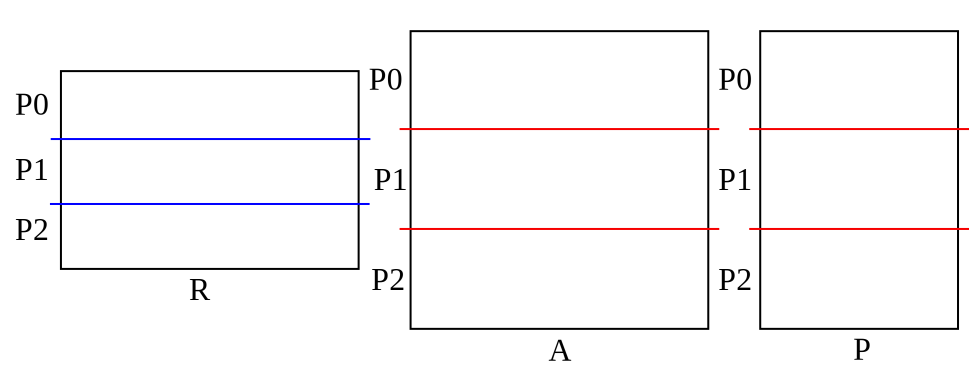
\includegraphics[width=8cm,height=3cm]{./figures/partition.pdf}
 \caption{}
 \label{fig:partition}
\end{figure}

\subsection{Part 1}

We assume the same partition of rows of $A$ on its columns. The same partition of rows of $R$ is assumed on columns of $P$ (Figure~\ref{fig:part1}).

\begin{figure}[tbh]
 \centering
 \includegraphics[width=5.5cm,height=3cm]{./figures/part1.pdf}
 \caption{}
 \label{fig:part1}
\end{figure}

Here we consider doing \matmult on processor $P1$. To perform \matmult, each block of $A$ on $P1$ should be multiplied by the blocks of $P$ with the same color (Figure~\ref{fig:part1b}).

\begin{figure}[tbh]
 \centering
 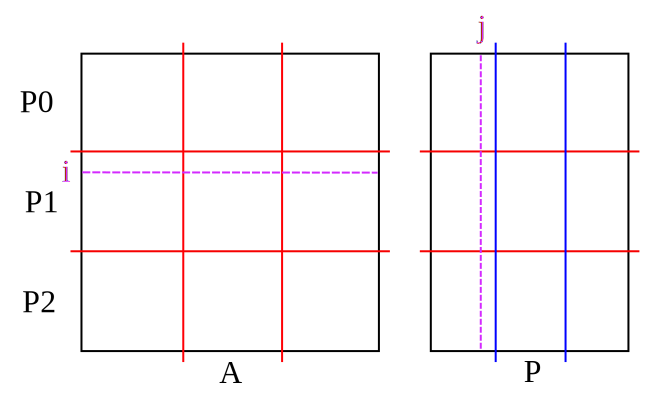
\includegraphics[width=5.5cm,height=3cm]{./figures/part1b.pdf}
 \caption{}
 \label{fig:part1b}
\end{figure}


\subsection{Part 2}
